%----------------------------------------------------------------------------------------
%	PACKAGES AND OTHER DOCUMENT CONFIGURATIONS
%----------------------------------------------------------------------------------------

\documentclass[12pt]{article} % Default font size is 12pt, it can be changed here

\usepackage{geometry} % Required to change the page size to A4
\geometry{a4paper} % Set the page size to be A4 as opposed to the default US Letter

\usepackage{graphicx} % Required for including pictures

\usepackage{float} % Allows putting an [H] in \begin{figure} to specify the exact location of the figure
\usepackage{wrapfig} % Allows in-line images such as the example fish picture
\usepackage{psfrag,amsmath,amsfonts,amsthm,amssymb,cite}
\usepackage{lipsum} % Used for inserting dummy 'Lorem ipsum' text into the template

\linespread{1.2} % Line spacing

%\setlength\parindent{0pt} % Uncomment to remove all indentation from paragraphs

\graphicspath{{Pictures/}} % Specifies the directory where pictures are stored

\begin{document}

%----------------------------------------------------------------------------------------
%	TITLE PAGE
%----------------------------------------------------------------------------------------

\begin{titlepage}

\newcommand{\HRule}{\rule{\linewidth}{0.5mm}} % Defines a new command for the horizontal lines, change thickness here

\center % Center everything on the page

\textsc{\LARGE CS4516: Project Methodology}\\[1.5cm] % Name of your university/college

\HRule \\[0.4cm]
{ \huge \bfseries Tag-Based IP Spoofing Prevention Under Low Deployment Scenarios}\\[0.4cm] % Title of your document
\HRule \\[1.5cm]

\begin{minipage}{0.4\textwidth}
\begin{flushleft} \large
\emph{Author:}\\
Michael Calder\\
Daniel Robertson\\
\end{flushleft}
\end{minipage}
~
\begin{minipage}{0.4\textwidth}
\begin{flushright} \large
\emph{Supervisor:} \\
Dr. Craig Shue % Supervisor's Name
\end{flushright}
\end{minipage}\\[4cm]

{\large \today}\\[3cm] % Date, change the \today to a set date if you want to be precise

%\includegraphics{Logo}\\[1cm] % Include a department/university logo - this will require the graphicx package

\vfill % Fill the rest of the page with whitespace

\end{titlepage}

%----------------------------------------------------------------------------------------
%	TABLE OF CONTENTS
%----------------------------------------------------------------------------------------

%\tableofcontents % Include a table of contents

\newpage % Begins the essay on a new page instead of on the same page as the table of contents 


%----------------------------------------------------------------------------------------
% -- Paper Outline --
% Detail NS-3 implementation of extended protocol, including class and file names. [drob]
% Explain hash-chain and TOTP-based implementation of tag transport [calder]
% Compare and contrast choice of hashing algorithms [calder]
% Talk about hash/security evaluation plan (testing for preimage resistance, ect).[drob]
%----------------------------------------------------------------------------------------

\section{Implementation of our extended protocol with NS-3}

Our implementation and evaluation is done through the Network Simulator 3 (NS-3) framework. NS-3 is an extensive open source framework for network testing and simulation, written in C++ with Python bindings for higher level scripting. It's seen wide spread use in both commercial and academic pursuits. After learning the NS-3 way of doing things, implementing a novel networking protocol is relatively straight forward. As was the case with this project, simply forking the repository, and extending a few base classes with the desired functionality, allows for rapid development.

\begin{figure}[ht!]
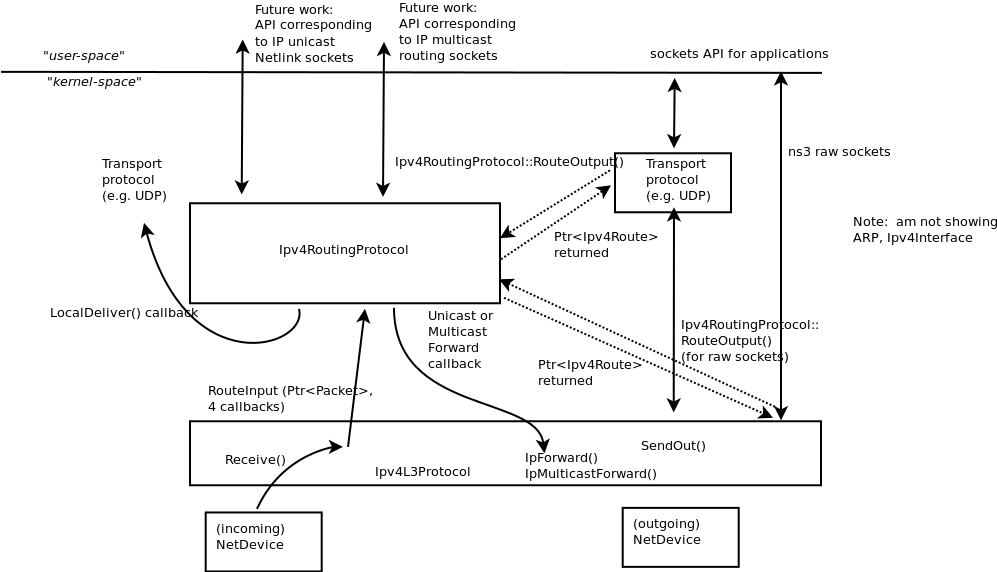
\includegraphics[width=160mm]{routing.png}
\caption{NS-3 {\it Ipv4RoutingProtocol} diagram. Note the interaction between the simulated layer's through RouteInput and RoutOutput\cite{ns-3-routing}}
\end{figure}

Since our extended protocol operates on the network layer, we worked mainly with NS-3's {\it Ipv4RoutingProtocol} interface. We extended the Ipv4GlobalRouting implementation in order to perform the necessary tag protocol logic on a per packet level. The {\it Ipv4RoutingProtocol} expects a RouteInput and RouteOutput function to be specified, which handles the control logic of prefix matching and packet forwarding. Here, we created a tag table as specified in \cite{Shue20081567}. Since our project's focus is more on the exchange of tagged packets over an insecure connection, we assumed that each router's tag table would already be populated. We do this by deterministically calculating a router's tag based off its associated prefix and incoming interface. This allows each router to act as though it's been fully configured, without the added implementation of tag discovery. 

Tags are stored within each packets header as a a list of tag objects. Necessary interaction functions (add, get, remove) were added to the {\it ipv4-header} class to support the addition of a tag field. The RouteInput and RouteOutput hooks both receive a Packet and Header pointer, allowing for this tag data to be accessed and modified by each router in the stream. 

These modifications are still insufficient to emulate our extended protocol in an actual deployment simulation. At it's core, an NS-3 simulation manages a group of configurable objects called {\it Nodes}. A Node can act as an end host, but can also be further extended to include a {\it NetDevice} (analogous to an NIC) in order to function as a router. {\it Nodes} are allocated and managed by {\it NodeContainers}. We use these containers to logically divide multiple {\it Nodes} into Subnets, each with their own tag. The SubNets are each connected to each other over {\it PointToPoint} links. Each router node is configured before simulation start up by the {\it GlobalRouteManager} class. We hooked into the configuration process in this class to control the deployment status of our extended protocol on each router. Each node manages an instance of the {\it GlobalRouter} class (which uses the {\it Ipv4GlobalRoutingProtocol}), which allows it to function as a Router. The extended protocol is disabled by default in our modified {\it Ipv4GlobalRoutingProtocol} class, so it must be manually enabled via the {\it GlobalRouter}. Since the GlobalRouteManager maintains all of the {\it GlobalRouters}, it has the responsibility of flipping the deployment switch.

With a stable modified implementation of the {\it Ipv4RoutingProtocol} and its constituent classes, we will set up a small topology consisting of multiple different subnets. Here, we will focus on the generation and verification of secured packet tags, based off of a router's base tag. We devise two core approaches, both of which involve computing the hash of a base tag in order to combine it with the current unix time interval. Both these approaches aim to vary the output tag that is to be transfered over an insecure channel, such that an attacker who obtains it cannot use it to spoof routers inside its originating subnet.

We will be testing both the speed and security of two different approaches to preventing tags from being compromised. For each of these approaches, we will use and compare both the fastest known non-cryptographic hash function (xxHash\cite{xxhash}) and the fastest known cryptographic function (MD5). 

The first approach is hash-chaining, which involves producing a series of hashes of the original tag to be used each day (changing the seed each day so that no two days have the same hash series). Every hash is the previous digest hashed again. If the time interval that these hashes change each day is 30 seconds, then we will need to produce 2,280 hashes to be stored in the router's RAM each day. We will test how long it takes to brute-force each hash algorithm to decide the maximum time interval that can be used and still render a compromised hash useless after its time interval has ended. We will measure how reasonable the needed memory is for each algorithm and how long it takes for routers to produce each day's chain. We note that for this approach, xxHash is a more attractive option, as it would allow large chains of small 32 bit hashes to be computed relatively quickly.

The second approach is inspired by TOTP (Time-based One-time Password). We will combine the current time (rounded to some interval like 30 seconds) with the original tag and then hash that result, rendering compromised hashes only useful for a small time interval. Security is a more important factor in this approach because given a time in addition to the hash algorithm, an attacker may be able to obtain the original tag. We will analyze the pre-image resistance of the output using a traditional brute-force approach, in order to determine the resilience of the approach. Clearly, it should be computationally difficult to derive the base tag from a hashed tag, when given the time interval used at the time of hashing, and the hash function its self. This calls for a cryptographic hash function, so we anticipate that MD5 and stronger cryptographic functions will be more secure. 




%----------------------------------------------------------------------------------------
%	BIBLIOGRAPHY
%----------------------------------------------------------------------------------------

\bibliography{references.bib}
\bibliographystyle{plain}

%----------------------------------------------------------------------------------------

\end{document}
